\documentclass[a4paper]{ctexart}
	\usepackage{geometry}
	\usepackage{enumerate}
	\usepackage{ntheorem}
	\usepackage{tikz}
	\usepackage{slashbox}
	\usepackage{tabularx}
	\usetikzlibrary{calc}
	\usepackage[fleqn]{amsmath}
	\geometry{left=3.18cm,right=3.18cm,top=2.44cm,bottom=2.44cm}
	\title{I - 方老师统治世界}
	\author{何柱}
	\allowdisplaybreaks
\begin{document}
	\maketitle
	凸包可以通过增量法计算得出。可以证明以下三点:
	\begin{enumerate}
		\item 连接两个不相交的凸包的最短线段中存在一条至少包含一个凸包上的一个点的线段。
		\item 连接被直线$x=0$分隔的两个凸包的最短距离等于连接左边凸包的右半壳和右边凸包的左半壳的最短距离。
		\item 在直线$x=0$左边的一个点到在直线$x=0$右边的一个凸包的左半壳的某个点的距离关于这个点的$y$坐标的函数为凹函数。
	\end{enumerate}

	于是,我们可以先算出左边的凸包的右半壳和右边的凸包的左半壳,由第一点和第二点可知,两个凸包的最短距离为左壳的点集到右壳的边集的最短距离和右壳的点集到左壳的边集的最短距离的较小值。由第三点可知,可以动态的从上一个边往距离小的方向遍历。问题到此就解决了。
	\begin{figure}[h]
		\begin{center}
			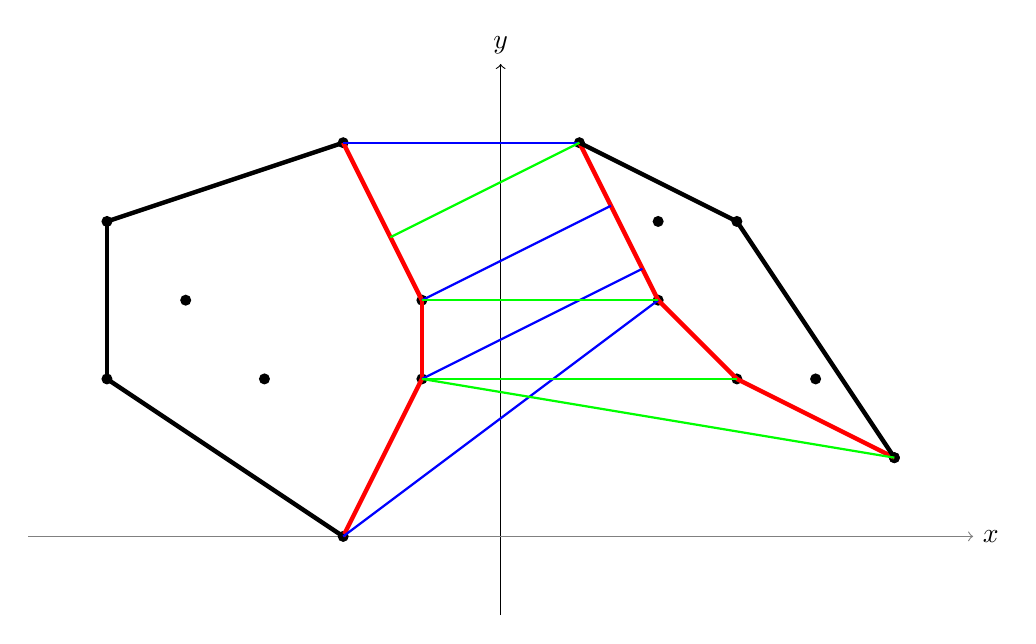
\begin{tikzpicture}
				\draw [thin, ->] (0,-1) -- (0,6)
				node [above, black] {$y$};
				\draw [thin, gray, ->] (-6,0) -- (6,0)
				node [right, black] {$x$};
			    \fill (-1, 3) coordinate (a_0) circle (2pt);
			    \fill (-1, 2) coordinate (a_1) circle (2pt);
			    \fill (-2, 5) coordinate (a_2) circle (2pt);
			    \fill (-2, 0) coordinate (a_3) circle (2pt);
			    \fill (-5, 2) coordinate (a_4) circle (2pt);
			    \fill (-4, 3) coordinate (a_5) circle (2pt);
			    \fill (-5, 4) coordinate (a_6) circle (2pt);
			    \fill (-3, 2) coordinate (a_7) circle (2pt);
			    \fill (4, 2) coordinate (b_0) circle (2pt);
			    \fill (5, 1) coordinate (b_1) circle (2pt);
			    \fill (3, 4) coordinate (b_2) circle (2pt);
			    \fill (3, 2) coordinate (b_3) circle (2pt);
			    \fill (2, 3) coordinate (b_4) circle (2pt);
			    \fill (1, 5) coordinate (b_5) circle (2pt);
			    \fill (2, 4) coordinate (b_6) circle (2pt);
			    \fill (5, 1) coordinate (b_7) circle (2pt);
				\draw [draw=red,ultra thick] (a_0) -- (a_1);
				\draw [draw=red,ultra thick] (a_1) -- (a_3);
				\draw [ultra thick] (a_3) -- (a_4);
				\draw [ultra thick] (a_4) -- (a_6);
				\draw [ultra thick] (a_6) -- (a_2);
				\draw [draw=red,ultra thick] (a_2) -- (a_0);
				\draw [draw=red,ultra thick] (b_5) -- (b_4);
				\draw [draw=red,ultra thick] (b_4) -- (b_3);
				\draw [draw=red,ultra thick] (b_3) -- (b_7);
				\draw [ultra thick] (b_7) -- (b_2);
				\draw [ultra thick] (b_2) -- (b_5);
				\draw [draw=blue,thick] (a_2) -- (b_5);
				\draw [draw=blue,thick] (a_0) -- ($(b_4)!(a_0)!(b_5)$);
				\draw [draw=blue,thick] (a_1) -- ($(b_4)!(a_1)!(b_5)$);
				\draw [draw=blue,thick] (a_3) -- (b_4);
				\draw [draw=green,thick] (b_5) -- ($(a_2)!(b_5)!(a_0)$);
				\draw [draw=green,thick] (b_4) -- ($(a_0)!(b_4)!(a_1)$);
				\draw [draw=green,thick] (b_3) -- (a_1);
				\draw [draw=green,thick] (b_7) -- (a_1);
			\end{tikzpicture}
		\end{center}
		\caption{一个示例,红线代表左壳和右壳,蓝线代表左壳的每个点到右壳的最短路,绿线代表右壳的每个点到左壳的最短路。}
	\end{figure}
\end{document}